% !TeX program = pdflatex
%
% Generated by scripts/build_latex.py from manuscript.json.
% Prose may be edited here; the tables are regenerated from the analysis, so put
% numeric corrections in the analysis rather than in this file.
%
% Target journal: Journal of Imaging Informatics in Medicine (Springer).
%
\documentclass[11pt,a4paper]{article}

\usepackage[utf8]{inputenc}
\usepackage[T1]{fontenc}
\usepackage{mathptmx}                 % Times text and math; on every TeX install
\usepackage[scaled=0.92]{helvet}
\usepackage[margin=1in]{geometry}
\usepackage{setspace}
\usepackage{graphicx}
\usepackage{booktabs}
\usepackage{longtable}
\usepackage{adjustbox}               % shrinks a table only when it is wider than the text
\usepackage{caption}
\usepackage[hidelinks]{hyperref}
\usepackage{lineno}
\usepackage{xcolor}

\captionsetup{font=small,labelfont=bf,justification=justified,singlelinecheck=false}
\renewcommand{\arraystretch}{1.12}
\setlength{\tabcolsep}{5pt}
\setcounter{secnumdepth}{2}

% Comment out for the camera-ready version.
\linenumbers
\doublespacing

\begin{document}

\begin{center}
{\Large\bfseries Label composition explains whether histology outperforms routine clinicopathological variables: a controlled comparison of four breast cancer risk signatures\par}
\vspace{1em}
{\normalsize Yaqeen Ali$^{1,2,3}$, Johannes Gregori$^{1,3}$\par}
\vspace{0.4em}
{\small\itshape 1 Darmstadt University of Applied Sciences, Darmstadt, Germany\par}
{\small\itshape 2 Doctoral Center Applied Informatics, Darmstadt, Germany\par}
{\small\itshape 3 mediri GmbH, Heidelberg, Germany\par}
{\small Corresponding author: Yaqeen Ali (\href{mailto:yaqeenali786@gmail.com}{yaqeenali786@gmail.com})\par}
{\small\itshape Submitted to JCO Clinical Cancer Informatics as an Original Report.\par}
\end{center}
\vspace{0.6em}

\section*{Abstract}
\begin{spacing}{1.35}
\noindent\textbf{PURPOSE} Deep learning on hematoxylin and eosin sections predicts the Oncotype DX recurrence score beyond routine clinicopathological variables, but whether this extends to other genomic risk signatures is untested under a common design. We hypothesized that the margin by which histology outperforms routine variables is governed by label composition --- how much of each binary label estrogen receptor (ER) status already explains --- a property of the target, not of the imaging model.\par\smallskip
\noindent\textbf{METHODS} Recomputed Oncotype DX, MammaPrint, and PAM50 ROR-S and ROR-P signatures were predicted from UNI patch embeddings by gated-attention multiple-instance learning in 82 patients from The Cancer Genome Atlas, under one shared five-fold partition and configuration, and compared on identical folds by paired bootstrap against ER status alone and a six-variable clinicopathological model. Label composition was quantified as the area under the curve (AUC) of ER status alone against each label.\par\smallskip
\noindent\textbf{RESULTS} Discrimination against chance ranged from AUC 0.744 to 0.892, but the margin over the clinicopathological model ran in almost the opposite order: Oncotype +0.280 (95\% CI, 0.133 to 0.435), ROR-P +0.160 (0.012 to 0.300), ROR-S +0.124 (0.013 to 0.246), and MammaPrint $-$0.042 ($-$0.134 to 0.034); only Oncotype survived multiplicity adjustment. The ordering was that of the ER-alone AUC (0.582, 0.610, 0.672, and 0.850), as the score definitions predict; the margin fell monotonically with that AUC across seven label definitions and was stable across five partition draws. A pre-extracted radiomic feature arm on the same folds showed non-nested selection inflating AUC by up to 0.121.\par\smallskip
\noindent\textbf{CONCLUSION} Whether histology outperforms routine clinicopathological variables is predictable from the labels alone. Studies predicting genomic signatures from images should report label composition and benchmark against clinicopathological variables, not chance.\par\smallskip
\end{spacing}
\vspace{0.5em}
\noindent\textbf{Keywords} Computational pathology $\cdot$ Multiple instance learning $\cdot$ Breast cancer $\cdot$ Gene expression signatures $\cdot$ Model benchmarking $\cdot$ Cross-validation
\clearpage

\section{Introduction}
Multigene expression assays guide adjuvant treatment in early-stage breast cancer. The 21-gene recurrence score (Oncotype DX) [1] and the 70-gene signature (MammaPrint) [2] identify patients in whom chemotherapy can be safely omitted, as shown prospectively by TAILORx [3] and MINDACT [4], and the PAM50 risk-of-recurrence scores provide subtype-based and proliferation-weighted estimates [5]. Cost and turnaround time limit access.

Deep learning on hematoxylin and eosin (H\&E) whole-slide images recovers hormone receptor status, HER2 status and intrinsic subtype [6--8]. For Oncotype DX the question is largely settled: Goyal et al reported an image model at AUC 0.87 against a clinicopathological model's 0.83 in 950 patients with external validation in 405 [9]; Boehm et al, in 6,172 patients, reported AUC 0.89 for a multimodal model against 0.73 for a clinicopathological nomogram [10]; and Shamai et al, with a multimodal model fine-tuned on the TAILORx trial and validated in six external cohorts, reported AUC 0.898 for high genomic risk [11]. Morphology carries recurrence-score information routine variables do not.

Whether this generalizes across signatures is not known, and the construction of the scores suggests that it should not. The recurrence score weights a five-gene proliferation group most heavily and enters a four-gene ER group with a negative coefficient [1]; in a predominantly ER-positive cohort, ER-group expression varies little between patients, so the variation that decides the High or Intermediate versus Low call is largely proliferative and only weakly tied to ER status. The 70-gene signature classifies by correlation with a good-prognosis profile that ER-negative tumors rarely meet --- in MINDACT, hormone receptor--negative tumors were almost uniformly genomically high risk [4] --- so its binary label in a mixed cohort is close to a restatement of ER status. The PAM50 scores lie between: the subtype-only score (ROR-S) draws on correlation with the basal-like and HER2-enriched centroids, which track ER-negative disease, whereas the proliferation-weighted score (ROR-P) adds within-luminal variation that is independent of ER status [5]. Because ER status is in every pathology report and visible on H\&E, a label that nearly restates it offers an image model little to learn that a clinician does not already have, however high the AUC. The expected ordering of the histology margin over routine variables therefore follows from the score definitions alone --- smallest for MammaPrint, intermediate for ROR-S, largest for ROR-P and Oncotype --- whereas its magnitude does not.

Testing this requires a constant design, and two common choices prevent it. Selecting hyperparameters separately for each target while held-out performance is visible turns the reported figure into the maximum over a search [12, 13], and evaluating targets on different partitions of the same patients confounds target with split; neither is detectable from a methods section. A second modality is available for this cohort: Li et al extracted 36 dynamic contrast-enhanced MRI radiomic features for the same patients [14]. We include them not to test whether MRI predicts the signatures but as a methodological control --- to measure, on the same folds, how much of an apparent radiomics signal is an artifact of the non-nested feature selection that such pipelines commonly use [15].

We therefore compared four recomputed signatures under one design --- one shared partition, one pre-fixed configuration, one model --- benchmarked each against ER status alone and a clinicopathological model, quantified label composition, tested whether histology adds to the clinical variables and measured the cost of non-nested selection in the radiomic feature arm.

\section{Methods}
\subsection{Study design and cohort}
This retrospective model-development study uses public, de-identified data and required no ethical approval; reporting follows TRIPOD+AI [16] (checklist in the Data Supplement). The cohort is the breast radiogenomics subset of The Cancer Genome Atlas [17] assembled by Li et al [14], for which recomputed signature scores have been published. Of 100 patients with recomputed scores, 83 also had a diagnostic whole-slide image with extracted features; one who had received neoadjuvant chemotherapy was excluded before any partition was drawn, leaving 82 (Fig S1). Follow-up comprises three recurrences and one death over a median of 42 months, so no survival or chemotherapy-benefit analysis is attempted.

\subsection{Prediction targets}
The targets are genefu-style recomputations from expression data [18] of the 21-gene recurrence score (GHI-RS), the 70-gene signature correlation (NKI70), and the PAM50 ROR-S and ROR-P scores. Binary labels follow the published group calls: GHI High or Intermediate versus Low; NKI70 Good versus Bad; ROR high or medium versus low. These are research recomputations, not commercial assay results or patient outcomes; every claim is at that level.

\subsection{Slide processing and model}
Whole-slide images were segmented, tiled into non-overlapping 256-pixel patches at 20$\times$ and encoded into 1,024-dimensional embeddings by the UNI foundation model [19] using the Trident toolkit [20]; this step was carried out beforehand as preparatory work in our group; no image processing method was developed here, and everything downstream was performed in this study. Each slide (median 19,376 patches, range 3,334 to 32,498) was reduced once, with a recorded seed, to a fixed pool of 512 patches, equalizing bag size and making evaluation deterministic (Fig 1a). A gated attention-based multiple-instance model [21] pools patch embeddings into a slide representation from which a regression head predicts the continuous score (Fig 1b); training details are in the Data Supplement.

\subsection{Partition and configuration}
A single five-fold partition was drawn by multi-label stratification [22], balanced on all four binary targets and on ER status, and used identically by every target (Fig 1c). An inner three-fold split, drawn the same way within each training set, supplied the validation fold: each outer fold trained on 42 to 44 patients, selected its epoch on 21 to 23 and was scored on 15 to 18 never seen during training or selection. The configuration was fixed before the confirmatory run and is the same for every target; it is the setting shared by the majority of four earlier per-target pipelines, which had been tuned with held-out performance visible, so the rule removes dependence on this study's measured performance and on target-specific tuning, not every prior look at the data.

\subsection{Comparators}
Two comparators were evaluated on the same folds. ER status alone is a single fixed binary predictor, oriented a priori so that ER-positive disease predicts the low-risk class, needing no fitting. The second is a six-variable logistic regression on age, ER, progesterone receptor and HER2 status, nodal status and ordinal AJCC stage --- the routine variables available here; grade and Ki-67 are not in the public extract --- L2-penalized at C = 1, pre-declared, trained on the remaining folds and used to predict each held-out fold. HER2 followed ASCO/CAP order [23]; one patient with uninformative HER2 testing is excluded from comparisons (n = 81). As a sensitivity analysis the penalty was instead chosen by inner cross-validation, and the apparent (in-sample) AUC was recorded. To test whether histology adds to rather than matches the clinical variables, the out-of-fold histology score was entered as a seventh variable into the tuned model, refitted inside each fold, and its association was also tested on the full data by likelihood-ratio test (odds ratio per SD); events per variable are reported for every fitted comparator [24].

\subsection{Pre-extracted radiomic feature arm}
The 36 DCE-MRI radiomic features of Li et al [14] were used as published; no image analysis was performed. Median imputation, standardization, univariate F-test filtering and L2-penalized logistic regression were fitted inside each training fold, with the number of features and the penalty chosen by inner cross-validation; the non-nested procedure, choosing them on all the data before the same cross-validation, was reproduced to measure its optimism. No clinicopathological comparator is reported for this arm, because the nested AUCs are at or near chance.

\subsection{Statistical analysis}
Label orientation was fixed a priori from the sign of the correlation between the continuous target and its binary label. Discrimination is reported as the AUC on pooled held-out predictions, with per-fold means and SDs alongside; pooling ranks every patient against every other, so a comparator refitted per fold can score below chance pooled but not per fold [25]. Confidence intervals are percentile intervals from 4,000 bootstrap resamples; differences between a model and a comparator use a paired bootstrap with a two-sided empirical p value, adjusted across the four targets by Holm's procedure [26]. Label composition is the AUC of ER status alone against each label (the balanced accuracy of ER as a classifier of it), with Cohen's $\kappa$ alongside, both model-free; proportion agreement is not used because prevalence dominates it. Three alternative binarization cuts of the same scores were evaluated on the same predictions. The whole pipeline was rerun under five independently drawn partitions, as in our earlier multi-seed evaluations [27], to measure how much the estimates move with the split. The minimum detectable difference between two AUCs on the same patients was computed from the Hanley--McNeil standard error [28, 29] (assumptions in the Data Supplement). Analyses used Python 3.11, PyTorch 2.14, scikit-learn 1.8 and statsmodels 0.15.

\section{Results}
\subsection{Cohort}
The 82 analyzed patients had a median age of 53 years (IQR 45 to 63); 71 (87\%) were ER-positive, 65 (79\%) HER2-negative and 65 (79\%) PR-positive; 41 (50\%) were node-positive; 71 (87\%) had invasive ductal carcinoma; and 53 (65\%) were PAM50 luminal A (Table 1).

\subsection{Discrimination against chance}
All four models discriminated against chance: pooled held-out AUC was 0.892 for MammaPrint, 0.834 for ROR-S, 0.815 for ROR-P and 0.744 for Oncotype, with Pearson correlations to the continuous score of 0.766, 0.695, 0.589 and 0.449 (Table 2; calibration and per-fold stability in Table S1).

\subsection{Discrimination against routine clinicopathological variables}
Against the pre-declared clinical model the ordering nearly reverses (Table 2, Fig 2a). That model alone reached out-of-fold AUC 0.464 for Oncotype, 0.655 for ROR-P, 0.710 for ROR-S and 0.934 for MammaPrint. Oncotype gains the most, +0.280 AUC (95\% CI, 0.133 to 0.435; p < 0.001), followed by ROR-P at +0.160 (0.012 to 0.300; p = 0.036) and ROR-S at +0.124 (0.013 to 0.246; p = 0.028). After Holm adjustment only the Oncotype margin remains significant (p = 0.001; ROR-P and ROR-S p = 0.084). MammaPrint gains nothing: $-$0.042 ($-$0.134 to 0.034; p = 0.313), so the clinicopathological model numerically exceeded the imaging model and the interval excludes any gain larger than 0.034. With the penalty tuned by inner cross-validation (Table 3, Fig 2a) the margins were +0.249 (0.090 to 0.416; p = 0.002), +0.173 (0.025 to 0.314; p = 0.020), +0.088 ($-$0.012 to 0.194; p = 0.090) and $-$0.042: the same conclusions under either comparator.

The Oncotype comparator is below chance under both penalties (per-fold 0.427 $\pm$ 0.269 when tuned) although its apparent AUC on all 81 patients is 0.721: six variables estimated from 14 minority-class cases fit the training folds and carry nothing to the held-out ones. The routine variables contain no transferable information about the Oncotype label here; they do not predict it inversely.

\subsection{Incremental value over the clinicopathological model}
Outperforming the clinical variables is not the same as adding to them (Table 3). For ROR-P the combined model improved on the clinical model by +0.138 AUC (0.014 to 0.262; p = 0.029; Holm p = 0.114) and the histology score remained strongly associated with the label after adjustment (odds ratio 3.35 per SD, 1.53 to 7.32; p < 0.001). For ROR-S the adjusted association was of the same size (3.34, 1.25 to 8.88; p = 0.007) but the cross-validated increment was small (+0.043, $-$0.020 to 0.114; p = 0.198). For Oncotype and MammaPrint the question is not answerable: with 14 minority-class cases a seven-variable model has two events per variable, the Oncotype combined model was no better than the clinical model ($-$0.020, $-$0.161 to 0.133) with an uninformative adjusted odds ratio (1.43, 0.66 to 3.07; p = 0.365), and the MammaPrint combined model matched a clinical model that already reaches AUC 0.934 ($-$0.016, $-$0.054 to 0.018). For those two targets only the head-to-head comparison is supported.

\subsection{Label composition}
The explanation for the ordering lies in the labels (Table 4, Fig 2b). ER status alone, as a fixed predictor, reaches AUC 0.850 against the MammaPrint label ($\kappa$ = 0.764), 0.672 against ROR-S ($\kappa$ = 0.388), 0.610 against ROR-P ($\kappa$ = 0.178) and 0.582 against Oncotype ($\kappa$ = 0.064) --- the order anticipated from the score definitions --- and the histology margin rises in exactly that order, from $-$0.042 to +0.280.

Because the published group calls are arbitrary cuts, three alternative cuts were evaluated on the same predictions. Moving the Oncotype cut to High versus Intermediate or Low leaves ER weakly informative (AUC 0.590, $\kappa$ = 0.098) and the margin large (+0.192, 0.058 to 0.340; p = 0.005). Moving the ROR cuts to high versus medium or low makes both labels far more ER-like --- ER alone reaches 0.740 against ROR-P ($\kappa$ = 0.511) and 0.826 against ROR-S ($\kappa$ = 0.726) --- and the margins collapse to +0.036 ($-$0.057 to 0.145; p = 0.493) and $-$0.030 ($-$0.094 to 0.025; p = 0.304) while raw discrimination against those labels rises to 0.897 and 0.928. Across all seven label definitions the margin falls monotonically as the AUC of ER alone rises. Seven points from one cohort do not establish a law; what they show is that label composition predicted whether histology outperformed routine variables here, and that changing one signature's cut moved it across that line.

\subsection{Within ER-positive disease, robustness, and the radiomic feature arm}
Within ER-positive, HER2-negative disease (n = 56) the clinicopathological model for Oncotype falls to AUC 0.279 (0.297 with tuned penalty) while the histology model retains 0.673; ROR-P is stable under restriction (0.815 to 0.756), ROR-S degrades (0.834 to 0.673), and MammaPrint is not evaluable because all 56 patients share one label (Table S2). Rerunning the whole pipeline under five independent partitions (Table S5) left the margin stable --- +0.213 $\pm$ 0.051 for Oncotype, +0.199 $\pm$ 0.045 for ROR-P, +0.111 $\pm$ 0.046 for ROR-S and $-$0.006 $\pm$ 0.048 for MammaPrint; the first three positive in all five draws, the last straddling zero (positive in two of five) --- so the ordering and the MammaPrint null are properties of the design, not of one split. In the radiomic feature arm, nested cross-validation gave AUC 0.588 to 0.637 with three of four intervals including chance, and the non-nested procedure inflated it by +0.022 to +0.121 (Table S3). The earlier per-target pipelines, with their own partitions and tuning, had ordered the targets differently under the same comparator (Table S4); the shared design reordered them without new data or a better model.

\section{Discussion}
Across four recomputed genomic risk signatures evaluated under one design, whether histology outperformed six routine clinicopathological variables varied from a margin of +0.280 AUC to none at all, and the variation tracked label composition, not the imaging model. Against the MammaPrint label, which ER status alone predicts at AUC 0.850 and which is single-class within ER-positive, HER2-negative disease, a model achieving AUC 0.892 was still numerically behind six routine variables --- a distinction invisible when performance is reported against chance. The direction was predictable from the score formulas, and the observed ordering of ER-alone AUC and of the histology margin is the predicted one; the magnitude was not predictable and is what the study measures.

Two questions are conflated easily. Whether an image model reaches the information in routine variables is a head-to-head comparison, which we pre-specified. Whether it adds to them needs a combined model, estimable at n = 81 only where the minority class allows: for the PAM50 scores the histology score stayed strongly associated after adjustment and for ROR-P the combined model also improved discrimination, whereas for Oncotype and MammaPrint, with 14 minority-class cases, neither the clinical nor a combined model can be estimated reliably, and our claims for those two targets are head-to-head claims only.

This complements the large Oncotype studies [9--11], which report a clear increment for the one signature whose label retains most variation within ER-positive disease, and suggests where the approach will not transfer. Three costless recommendations follow: report the AUC of receptor status alone against the binarized label, or $\kappa$, because it bounds what any model can contribute; benchmark against a clinicopathological model, not chance, and say whether the image model was compared with it or added to it; and when several targets are compared, share one partition and one configuration and nest all selection inside the training folds. The magnitudes involved are not a technicality: per-target partitioning and tuning reordered the four targets (Table S4), and in the radiomic feature arm --- included as a methodological control, not as a competitor to histology --- non-nested selection accounted for most of the apparent signal, showing that the selection bias long described in the literature [12, 13] and recently documented for pathology foundation models [30] is directly observable on the same data, at the 0.03 to 0.12 AUC scale at which increments are commonly reported.

\subsection{Limitations}
The targets are research recomputations of signature scores, not commercial assay results and not patient outcomes; with three recurrences and one death, no prognostic or chemotherapy-benefit claim is made; clinical utility rests on the cohorts cited above. The cohort is small: the minimum detectable difference between two AUCs on the same patients is 0.135 to 0.154 depending on class balance and 0.165 to 0.221 in the ER-positive, HER2-negative subgroup, so only the Oncotype margin survives adjustment, the ROR-P and ROR-S margins are suggestive until replicated, and the confidence intervals rest on one pre-declared partition --- stabilized but not narrowed by the five-partition repeat. The comparator lacks grade and Ki-67, so the Oncotype margin is against a weaker comparator than a full pathology report. Other limitations are the single cohort without external validation, a fixed 512-patch sample of each slide, a configuration inherited from pipelines that had seen these data, and the over-representation of ER-positive disease. The pathology-only arm can be extended to roughly 900 TCGA cases with no new data collection, at which point the minimum detectable difference falls to about 0.04 to 0.05 and the incremental question becomes answerable for every target.

In conclusion, whether deep learning on H\&E outperforms routine clinicopathological variables differs sharply between genomic risk signatures, and the difference was governed by label composition. Discrimination against chance is not an informative endpoint; studies should report label composition, benchmark against a clinicopathological model and say whether the image model was compared with it or added to it, and nest all selection inside the training folds.

\begin{spacing}{1.0}
\subsection*{Support}
[to complete]\par\smallskip
\subsection*{Authors' disclosures of potential conflicts of interest}
[to complete]\par\smallskip
\subsection*{Author contributions}
Conception and design: Yaqeen Ali, Johannes Gregori. Data processing, analysis and software: Yaqeen Ali. Manuscript writing: Yaqeen Ali. Critical revision and supervision: Johannes Gregori. Final approval: all authors.\par\smallskip
\subsection*{Acknowledgments}
We thank Vincenzo Della Mea (University of Udine) for providing the curated clinical data file for this cohort.\par\smallskip
\subsection*{Ethics}
Not required; the analysis uses public, de-identified data from The Cancer Genome Atlas.\par\smallskip
\subsection*{Data sharing statement}
Whole-slide images and clinical data are available through the NCI Genomic Data Commons and MRI data through The Cancer Imaging Archive; recomputed signature scores derive from published expression data [14]. All analysis code, the locked run manifest (seeds, configuration, package versions) and the derived result tables are available at [repository URL].\par\smallskip
\end{spacing}
\section*{References}
\begin{spacing}{1.0}
\begin{enumerate}\setlength{\itemsep}{2pt}
\item Paik S, Shak S, Tang G, et al: A multigene assay to predict recurrence of tamoxifen-treated, node-negative breast cancer. N Engl J Med 351:2817-2826, 2004
\item van 't Veer LJ, Dai H, van de Vijver MJ, et al: Gene expression profiling predicts clinical outcome of breast cancer. Nature 415:530-536, 2002
\item Sparano JA, Gray RJ, Makower DF, et al: Adjuvant chemotherapy guided by a 21-gene expression assay in breast cancer. N Engl J Med 379:111-121, 2018
\item Cardoso F, van 't Veer LJ, Bogaerts J, et al: 70-gene signature as an aid to treatment decisions in early-stage breast cancer. N Engl J Med 375:717-729, 2016
\item Parker JS, Mullins M, Cheang MCU, et al: Supervised risk predictor of breast cancer based on intrinsic subtypes. J Clin Oncol 27:1160-1167, 2009
\item Couture HD, Williams LA, Geradts J, et al: Image analysis with deep learning to predict breast cancer grade, ER status, histologic subtype, and intrinsic subtype. NPJ Breast Cancer 4:30, 2018
\item Naik N, Madani A, Esteva A, et al: Deep learning-enabled breast cancer hormonal receptor status determination from base-level H\&E stains. Nat Commun 11:5727, 2020
\item La Barbera D, Polónia A, Roitero K, et al: Detection of HER2 from haematoxylin-eosin slides through a cascade of deep learning classifiers via multi-instance learning. J Imaging 6:82, 2020
\item Goyal M, Marotti JD, Workman AA, et al: A multi-model approach integrating whole-slide imaging and clinicopathologic features to predict breast cancer recurrence risk. NPJ Breast Cancer 10:93, 2024
\item Boehm KM, El Nahhas OSM, Marra A, et al: Multimodal histopathologic models stratify hormone receptor-positive early breast cancer. Nat Commun 16:2106, 2025
\item Shamai G, Cohen S, Binenbaum Y, et al: Deep learning on histopathological images to predict breast cancer recurrence risk and chemotherapy benefit: a multicentre, model development and validation study. Lancet Oncol, 2026. doi:10.1016/S1470-2045(25)00727-2
\item Varma S, Simon R: Bias in error estimation when using cross-validation for model selection. BMC Bioinformatics 7:91, 2006
\item Cawley GC, Talbot NLC: On over-fitting in model selection and subsequent selection bias in performance evaluation. J Mach Learn Res 11:2079-2107, 2010
\item Li H, Zhu Y, Burnside ES, et al: MR imaging radiomics signatures for predicting the risk of breast cancer recurrence as given by research versions of MammaPrint, Oncotype DX, and PAM50 gene assays. Radiology 281:382-391, 2016
\item Tareke TW, Payan N, Cochet A, et al: Automated radiomics analysis from multi-modal image segmentation for predicting triple negative breast cancer. Annu Int Conf IEEE Eng Med Biol Soc, 2025. doi:10.1109/EMBC58623.2025.11252611
\item Collins GS, Moons KGM, Dhiman P, et al: TRIPOD+AI statement: Updated guidance for reporting clinical prediction models that use regression or machine learning methods. BMJ 385:e078378, 2024
\item The Cancer Genome Atlas Network: Comprehensive molecular portraits of human breast tumours. Nature 490:61-70, 2012
\item Gendoo DMA, Ratanasirigulchai N, Schr\"oder MS, et al: Genefu: An R/Bioconductor package for computation of gene expression-based signatures in breast cancer. Bioinformatics 32:1097-1099, 2016
\item Chen RJ, Ding T, Lu MY, et al: Towards a general-purpose foundation model for computational pathology. Nat Med 30:850-862, 2024
\item Zhang A, Jaume G, Vaidya A, et al: Accelerating data processing and benchmarking of AI models for pathology. arXiv:2502.06750, 2025
\item Ilse M, Tomczak JM, Welling M: Attention-based deep multiple instance learning. Proc Mach Learn Res 80:2127-2136, 2018
\item Sechidis K, Tsoumakas G, Vlahavas I: On the stratification of multi-label data. Lect Notes Comput Sci 6913:145-158, 2011
\item Wolff AC, Hammond MEH, Allison KH, et al: Human epidermal growth factor receptor 2 testing in breast cancer: American Society of Clinical Oncology/College of American Pathologists clinical practice guideline focused update. J Clin Oncol 36:2105-2122, 2018
\item Peduzzi P, Concato J, Kemper E, et al: A simulation study of the number of events per variable in logistic regression analysis. J Clin Epidemiol 49:1373-1379, 1996
\item Forman G, Scholz M: Apples-to-apples in cross-validation studies: Pitfalls in classifier performance measurement. ACM SIGKDD Explor Newsl 12:49-57, 2010
\item Holm S: A simple sequentially rejective multiple test procedure. Scand J Stat 6:65-70, 1979
\item Ali Y, M\"uller J, Weinmann A, et al: Performance of federated versus centralized learning for mammography classification across film-digital domain shift. Front Digit Health, 2026. doi:10.3389/fdgth.2026.1715858
\item Hanley JA, McNeil BJ: The meaning and use of the area under a receiver operating characteristic (ROC) curve. Radiology 143:29-36, 1982
\item Hanley JA, McNeil BJ: A method of comparing the areas under receiver operating characteristic curves derived from the same cases. Radiology 148:839-843, 1983
\item Akebli H, Della Mea V: Domain generalization of histopathology foundation models in multicenter, multi-scanner cohorts: A comparative benchmark. J Imaging 12:381, 2026
\end{enumerate}
\end{spacing}
\clearpage
\section*{Tables}
\begin{spacing}{1.0}
\small
\begin{longtable}{@{}p{0.40\textwidth}rrr@{}}
\caption*{\textbf{Table 1.} Cohort characteristics, overall and by the ROR-P label. Median [IQR] for age, n (\%) otherwise. HER2 follows ASCO/CAP order: FISH where informative, otherwise immunohistochemistry. No significance tests are reported, because the groups are defined by a computed score rather than by an exposure.}\\
\toprule
\textbf{Characteristic} & \textbf{All (n = 82)} & \textbf{ROR-P low (n = 32)} & \textbf{ROR-P high (n = 50)} \\
\midrule\endfirsthead
\toprule
\textbf{Characteristic} & \textbf{All (n = 82)} & \textbf{ROR-P low (n = 32)} & \textbf{ROR-P high (n = 50)} \\
\midrule\endhead
\textbf{Age at diagnosis, years} & 53 [45--63] & 52 [45--63] & 54 [46--62] \\
\textbf{Menopausal status} &  &  &  \\
\quad Postmenopausal & 43 (52\%) & 14 (44\%) & 29 (58\%) \\
\quad Premenopausal & 31 (38\%) & 13 (41\%) & 18 (36\%) \\
\quad Perimenopausal & 5 (6\%) & 3 (9\%) & 2 (4\%) \\
\quad Unknown & 2 (2\%) & 2 (6\%) & 0 (0\%) \\
\quad Indeterminate & 1 (1\%) & 0 (0\%) & 1 (2\%) \\
\textbf{ER status} &  &  &  \\
\quad Positive & 71 (87\%) & 32 (100\%) & 39 (78\%) \\
\quad Negative & 11 (13\%) & 0 (0\%) & 11 (22\%) \\
\textbf{PR status} &  &  &  \\
\quad Positive & 65 (79\%) & 31 (97\%) & 34 (68\%) \\
\quad Negative & 17 (21\%) & 1 (3\%) & 16 (32\%) \\
\textbf{HER2 status (ASCO/CAP)} &  &  &  \\
\quad Negative & 65 (79\%) & 26 (81\%) & 39 (78\%) \\
\quad Positive & 16 (20\%) & 5 (16\%) & 11 (22\%) \\
\quad Unknown & 1 (1\%) & 1 (3\%) & 0 (0\%) \\
\textbf{AJCC pathologic stage} &  &  &  \\
\quad Stage I & 15 (18\%) & 7 (22\%) & 8 (16\%) \\
\quad Stage IA & 3 (4\%) & 2 (6\%) & 1 (2\%) \\
\quad Stage II & 1 (1\%) & 0 (0\%) & 1 (2\%) \\
\quad Stage IIA & 35 (43\%) & 10 (31\%) & 25 (50\%) \\
\quad Stage IIB & 18 (22\%) & 10 (31\%) & 8 (16\%) \\
\quad Stage IIIA & 6 (7\%) & 3 (9\%) & 3 (6\%) \\
\quad Stage IIIC & 4 (5\%) & 0 (0\%) & 4 (8\%) \\
\textbf{Nodal status} &  &  &  \\
\quad Node negative & 41 (50\%) & 14 (44\%) & 27 (54\%) \\
\quad Node positive & 41 (50\%) & 18 (56\%) & 23 (46\%) \\
\textbf{Histology} &  &  &  \\
\quad Invasive ductal & 71 (87\%) & 26 (81\%) & 45 (90\%) \\
\quad Invasive lobular & 9 (11\%) & 4 (12\%) & 5 (10\%) \\
\quad Other & 1 (1\%) & 1 (3\%) & 0 (0\%) \\
\quad Mixed & 1 (1\%) & 1 (3\%) & 0 (0\%) \\
\textbf{PAM50 subtype} &  &  &  \\
\quad LumA & 53 (65\%) & 29 (91\%) & 24 (48\%) \\
\quad LumB & 10 (12\%) & 0 (0\%) & 10 (20\%) \\
\quad Her2 & 5 (6\%) & 0 (0\%) & 5 (10\%) \\
\quad Basal & 10 (12\%) & 0 (0\%) & 10 (20\%) \\
\quad Normal & 4 (5\%) & 3 (9\%) & 1 (2\%) \\
\bottomrule
\end{longtable}
\normalsize

\begin{table}[htbp]\centering\footnotesize
\caption*{\textbf{Table 2.} Primary endpoint: histology against chance, against ER status alone and against the pre-declared six-variable clinicopathological model (L2-penalized logistic regression, C = 1), all on pooled held-out predictions. ER alone is a fixed binary predictor oriented a priori (ER-positive predicts the low-risk class). n = 81 with complete covariates; paired bootstrap, 4,000 resamples; Holm adjustment across the four targets. Rows are ordered by the gain column, which runs in almost the opposite order to raw AUC.}
\begin{adjustbox}{max width=\textwidth}
\begin{tabular}{@{}lcccccc@{}}
\toprule
\textbf{Signature} & \textbf{Histology AUC (95\% CI)} & \textbf{ER alone} & \textbf{Clinical} & \textbf{Gain over clinical (95\% CI)} & \textbf{p} & \textbf{Holm p} \\
\midrule
Oncotype (GHI-RS) & 0.744 (0.631--0.846) & 0.582 & 0.464 & +0.280 (0.133 to 0.435) & <0.001 & 0.001 \\
PAM50 ROR-P & 0.815 (0.718--0.900) & 0.610 & 0.655 & +0.160 (0.012 to 0.300) & 0.036 & 0.084 \\
PAM50 ROR-S & 0.834 (0.727--0.921) & 0.672 & 0.710 & +0.124 (0.013 to 0.246) & 0.028 & 0.084 \\
MammaPrint (NKI70) & 0.892 (0.770--0.980) & 0.850 & 0.934 & $-$0.042 ($-$0.134 to 0.034) & 0.313 & 0.313 \\
\bottomrule
\end{tabular}
\end{adjustbox}\end{table}

\footnotesize
\begin{longtable}{@{}p{0.28\textwidth}rrrr@{}}
\caption*{\textbf{Table 3.} Sensitivity to the comparator, and incremental value (n = 81). Events per variable: minority class $\div$ 7, for a seven-term logistic model. Clinical model, penalty tuned: the six-variable model with its penalty chosen by inner three-fold cross-validation; the histology gain is against that comparator. Clinical model + histology score: the same model with the out-of-fold histology score as a seventh variable, refitted inside each fold, compared with the tuned clinical model. Adjusted association: odds ratio per SD of the histology score after adjustment for the six variables, fitted once on all 81 patients, with a likelihood-ratio test. Paired bootstrap, 4,000 resamples; Holm adjustment across the four targets.}\\
\toprule
\textbf{} & \textbf{Oncotype} & \textbf{ROR-P} & \textbf{ROR-S} & \textbf{MammaPrint} \\
\midrule\endfirsthead
\toprule
\textbf{} & \textbf{Oncotype} & \textbf{ROR-P} & \textbf{ROR-S} & \textbf{MammaPrint} \\
\midrule\endhead
\textbf{Events per variable} & 2.0 & 4.4 & 4.6 & 2.0 \\
\textbf{Clinical model, penalty tuned} &  &  &  &  \\
\quad AUC, pooled & 0.495 & 0.642 & 0.746 & 0.934 \\
\quad AUC per fold, mean $\pm$ SD & 0.427 $\pm$ 0.269 & 0.669 $\pm$ 0.142 & 0.735 $\pm$ 0.139 & 0.950 $\pm$ 0.056 \\
\quad Histology gain (95\% CI) & +0.249 (0.090 to 0.416) & +0.173 (0.025 to 0.314) & +0.088 ($-$0.012 to 0.194) & $-$0.042 ($-$0.134 to 0.034) \\
\quad p; Holm p & 0.002; 0.008 & 0.020; 0.060 & 0.090; 0.179 & 0.313; 0.313 \\
\textbf{Clinical model + histology score} &  &  &  &  \\
\quad AUC, pooled & 0.474 & 0.781 & 0.789 & 0.918 \\
\quad AUC per fold, mean $\pm$ SD & 0.563 $\pm$ 0.281 & 0.834 $\pm$ 0.121 & 0.818 $\pm$ 0.102 & 0.962 $\pm$ 0.054 \\
\quad Incremental gain (95\% CI) & $-$0.020 ($-$0.161 to 0.133) & +0.138 (0.014 to 0.262) & +0.043 ($-$0.020 to 0.114) & $-$0.016 ($-$0.054 to 0.018) \\
\quad p; Holm p & 0.755; 0.755 & 0.029; 0.114 & 0.198; 0.593 & 0.336; 0.671 \\
\textbf{Adjusted association, full data} &  &  &  &  \\
\quad Odds ratio per SD (95\% CI) & 1.43 (0.66 to 3.07) & 3.35 (1.53 to 7.32) & 3.34 (1.25 to 8.88) & 1.40 (0.33 to 5.91) \\
\quad Likelihood-ratio p; Holm p & 0.365; 0.731 & <0.001; 0.002 & 0.007; 0.020 & 0.640; 0.731 \\
\bottomrule
\end{longtable}
\normalsize

\begin{table}[htbp]\centering\footnotesize
\caption*{\textbf{Table 4.} Label composition --- how much of each binary label is ER status --- and the histology gain against it, for the four published group calls and three alternative cuts of the same scores (n = 81). AUC of ER alone is the balanced accuracy of ER status as a classifier of the label, with ER-positive assigned to the low-risk class a priori; $\kappa$ is Cohen's kappa for the same agreement. Both are properties of the label, computed without any model. Gain is against the pre-declared clinicopathological model. ``Alternative'': a cut of the same score other than the published group call, evaluated on the same predictions. Rows are ordered by the AUC of ER alone; the gain falls monotonically along them.}
\begin{adjustbox}{max width=\textwidth}
\begin{tabular}{@{}lccccc@{}}
\toprule
\textbf{Target} & \textbf{Binary label} & \textbf{Positive / negative} & \textbf{AUC of ER alone} & \textbf{$\kappa$ with ER} & \textbf{Gain over clinical; p} \\
\midrule
Oncotype & High or Intermediate vs Low & 67 / 14 & 0.582 & 0.064 & +0.280; <0.001 \\
Oncotype & High vs Intermediate or Low (alternative) & 61 / 20 & 0.590 & 0.098 & +0.192; 0.005 \\
ROR-P & high or medium vs low & 50 / 31 & 0.610 & 0.178 & +0.160; 0.036 \\
ROR-S & high or medium vs low & 32 / 49 & 0.672 & 0.388 & +0.124; 0.028 \\
ROR-P & high vs medium or low (alternative) & 13 / 68 & 0.740 & 0.511 & +0.036; 0.493 \\
ROR-S & high vs medium or low (alternative) & 15 / 66 & 0.826 & 0.726 & $-$0.030; 0.304 \\
MammaPrint & Good vs Bad & 67 / 14 & 0.850 & 0.764 & $-$0.042; 0.313 \\
\bottomrule
\end{tabular}
\end{adjustbox}\end{table}

\end{spacing}
\clearpage
\section*{Figures}
\begin{figure}[htbp]\centering
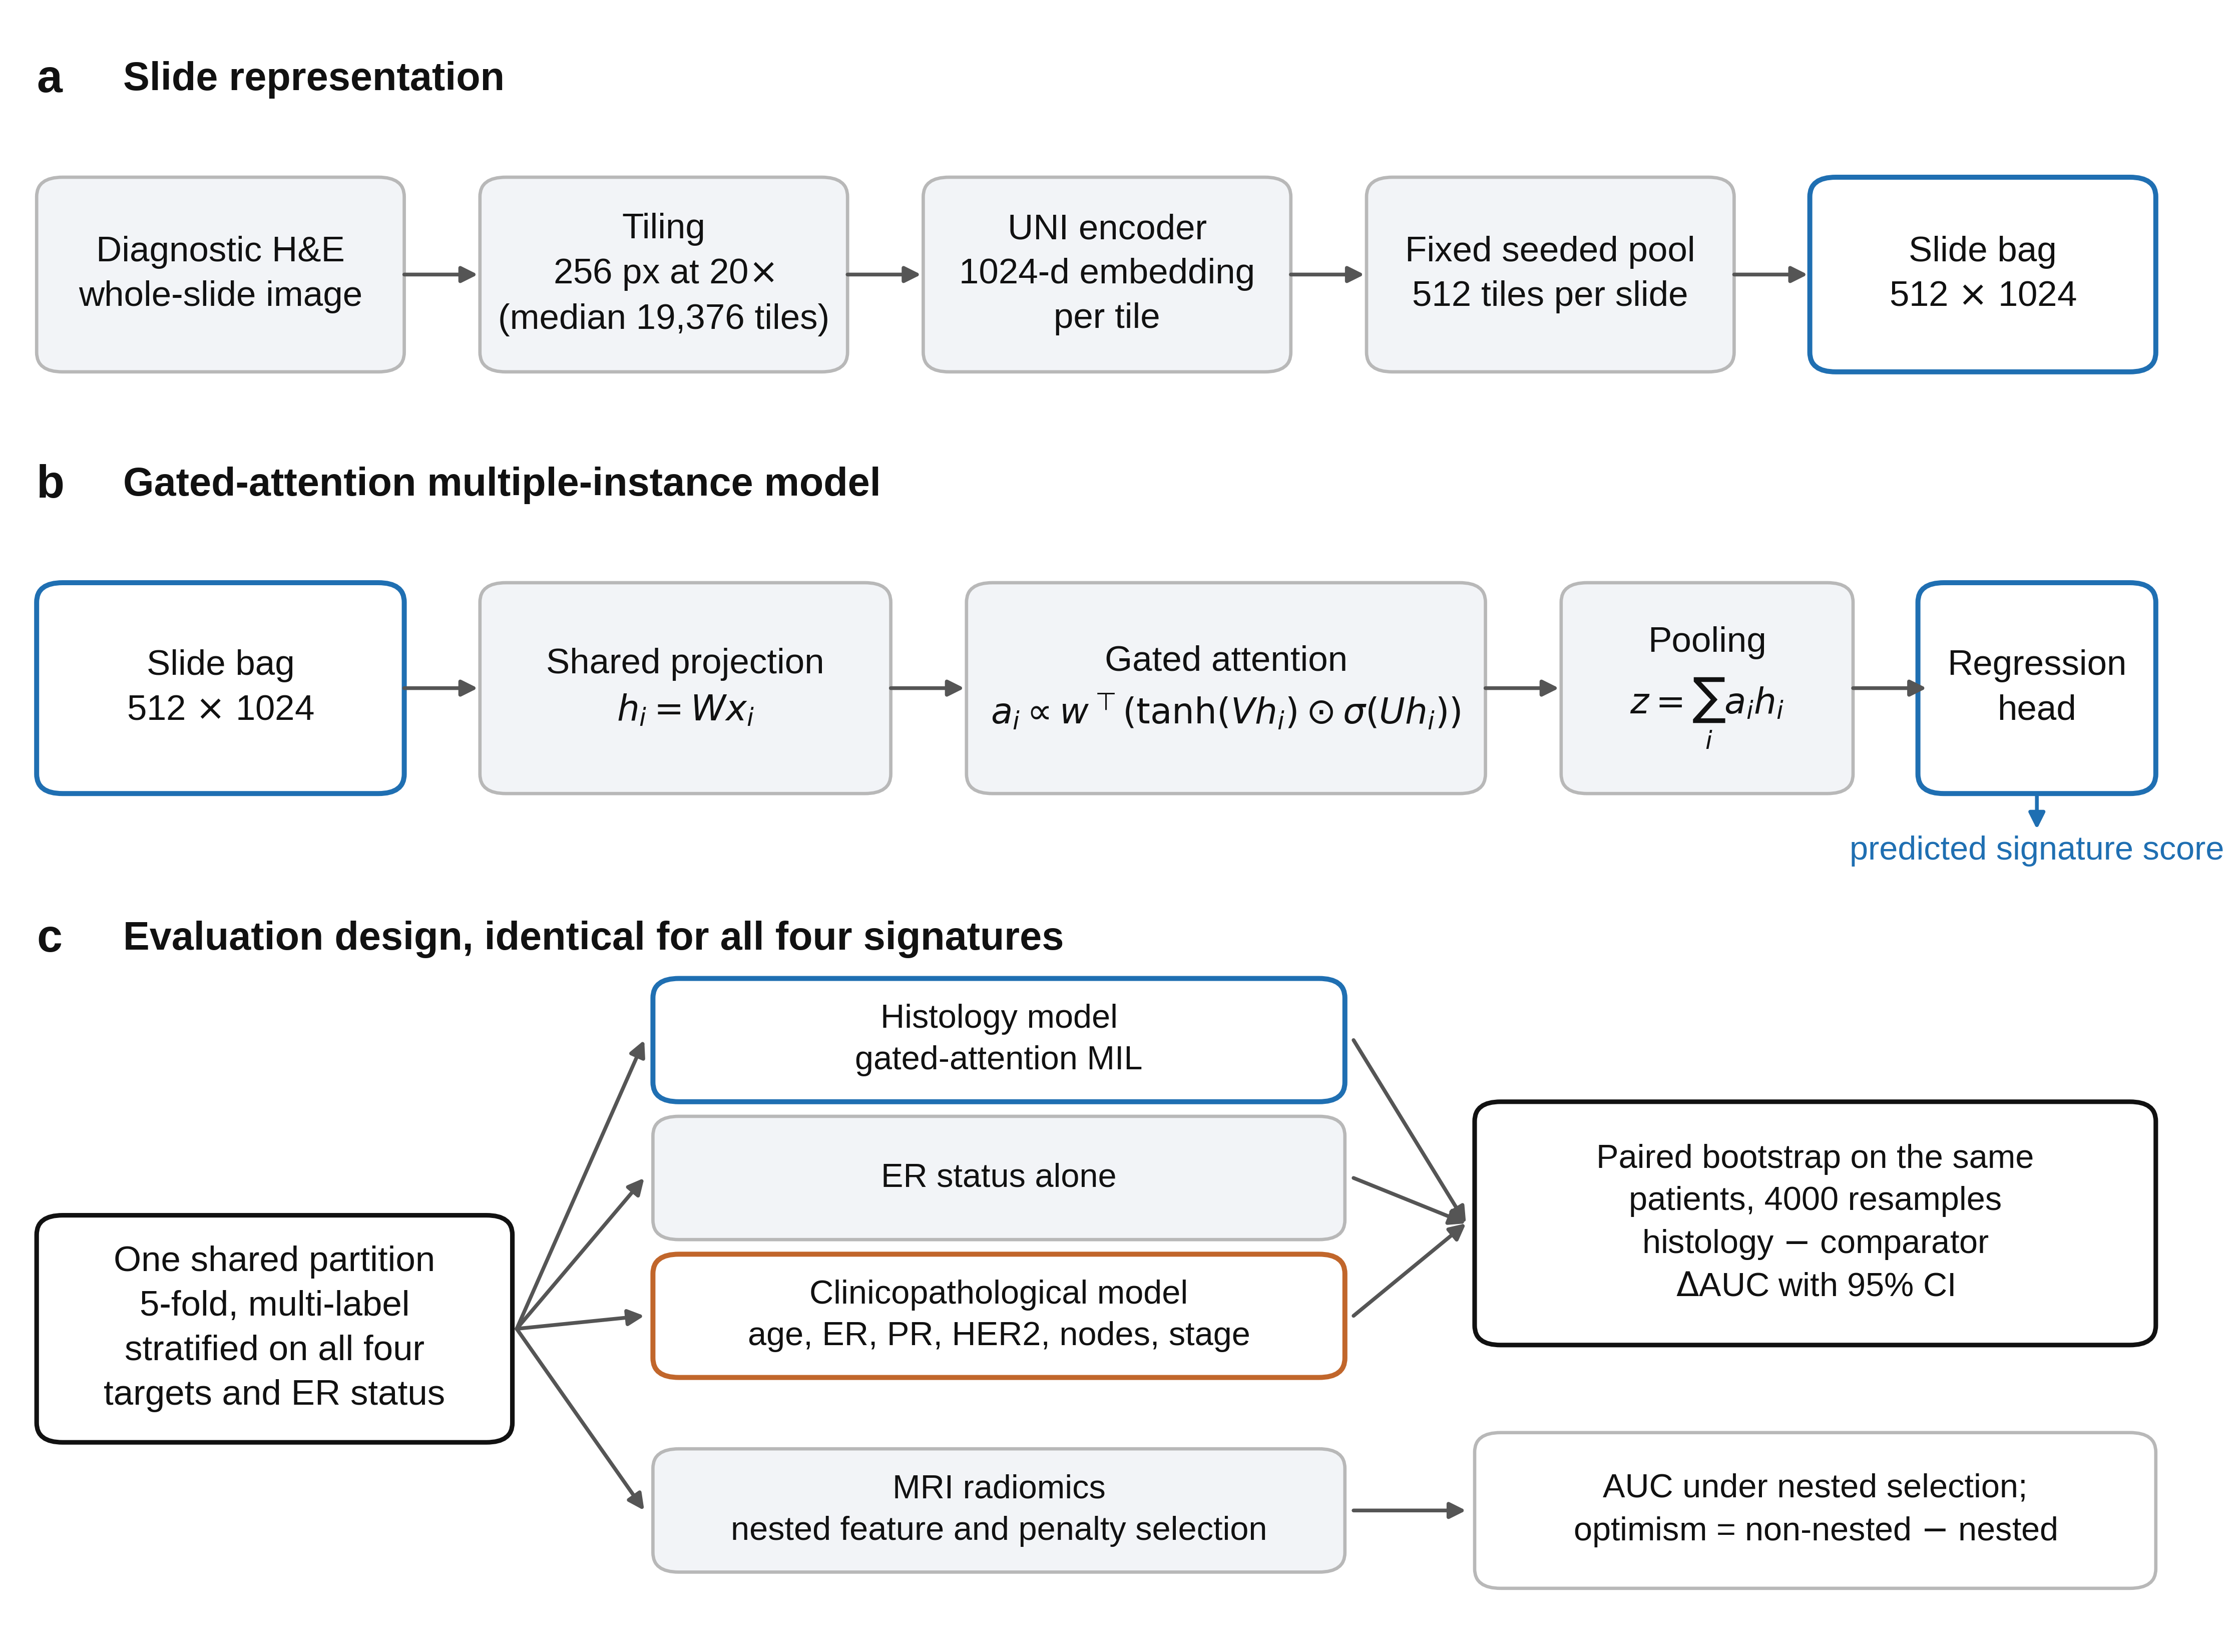
\includegraphics[width=0.95\textwidth]{figures/Fig1.png}
\caption*{\textbf{Fig 1.} Study design and model architecture. (a) Each diagnostic H\&E whole-slide image is tiled at 20$\times$ and encoded by the UNI foundation model, then reduced once, with a seed recorded per slide, to a fixed pool of 512 patches. (b) A gated-attention multiple-instance model weights patches and pools them into a slide representation from which the continuous signature score is predicted. (c) All four signatures use one shared multi-label stratified five-fold partition. Histology is compared on identical folds against ER status alone and against a six-variable clinicopathological model by paired bootstrap; the pre-extracted radiomic feature arm is evaluated on the same folds under nested selection, with the non-nested procedure reproduced to measure its optimism.}
\end{figure}
\clearpage
\begin{figure}[htbp]\centering
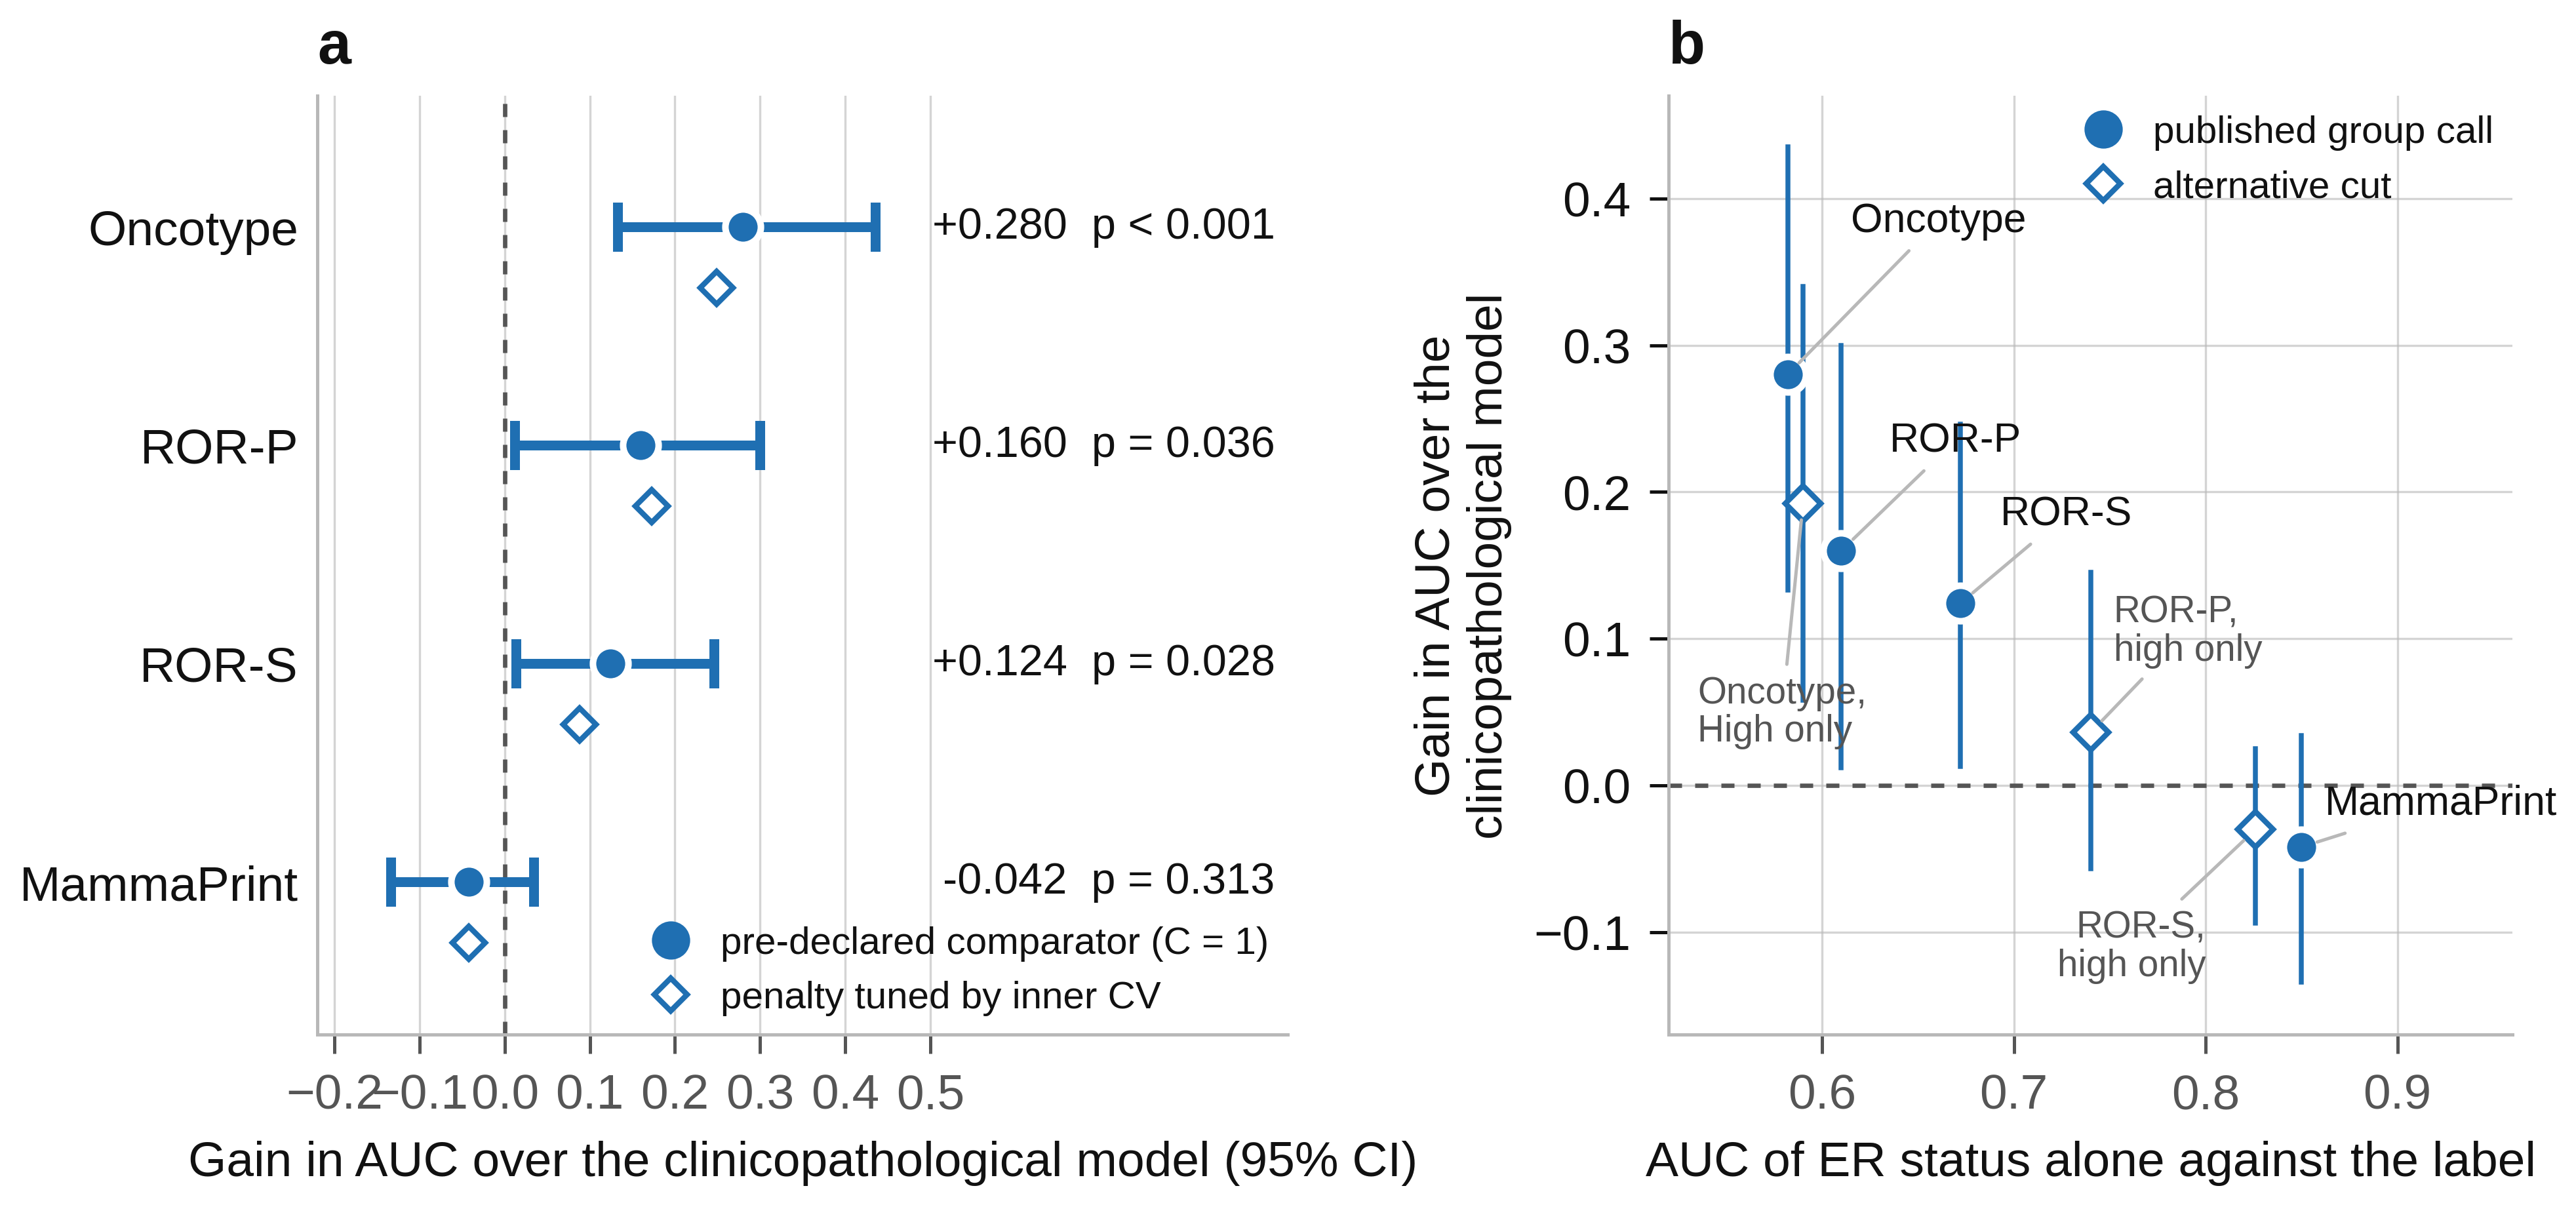
\includegraphics[width=0.95\textwidth]{figures/Fig2.png}
\caption*{\textbf{Fig 2.} The histology margin over the clinicopathological model, and what predicts it. (a) Gain in AUC over the six-variable model with 95\% percentile intervals from a paired bootstrap of 4,000 resamples (n = 81), for the pre-declared comparator (filled) and the comparator with its penalty tuned by inner cross-validation (open). (b) The same gain against the AUC of ER status alone as a fixed predictor of each label --- label composition --- for the four published group calls (filled) and three alternative cuts of the same scores (open); vertical bars are the 95\% intervals of the gain. The margin falls monotonically as the label becomes more nearly a restatement of ER status.}
\end{figure}
\clearpage
\end{document}
